\chapter{Methods}

\section{Creation of Synthetic Data}

\begin{figure}[htbp]
    \centering
    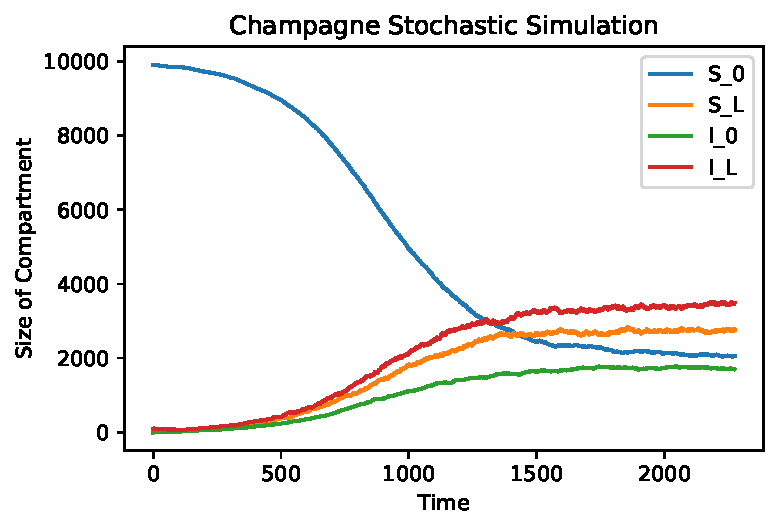
\includegraphics[width = \textwidth]{../champagne_GP_images/champagne_simulation.pdf}
    \caption{
        A Doob-Gillespie Simulation of the model described by
        \cite{champagne_using_2022} with $\alpha = 0.4,$ $\beta = 0.4,$
        $\gamma_L = 1 / 223,$ $\lambda = 0.04,$ $f = 1 / 72,$ $r = 1 / 60,$ and
        $\delta = 0.$ The population was 1000, with 10 initial infections
        (both blood and liver stage).
    }
    \label{fig:champ_doob}
\end{figure}

We investigated the model by \cite{champagne_using_2022} as described in
\ref{sec:champ_mod}. A malaria epidemic was simulated using the Doob-Gillepsie
algorithm (see Figure \ref{fig:champ_doob}), using a population
size of 1,000, and initial infected population of 10 (with both liver and blood
stage infection). The parameters used closely followed those reported in
\cite{champagne_using_2022}: \begin{itemize}
    \item effective blood stage treatment proportion $\alpha = 0.4,$
    \item effective liver stage treatment proportion $\beta = 0.4,$
    \item rate of liver stage disease clearance
          $\gamma_L = 1 / 223 \text{ days}^{-1},$
    \item importation rate $\delta = 0$ (assumed to be known),
    \item rate of infection $\lambda = 0.04 \text{ days}^{-1},$
    \item rate of relapse $f = 1 / 72 \text{ days}^{-1},$
    \item rate of blood stage disease clearance $r = 1 / 60 \text{ days}^{-1}.$
\end{itemize}

From intialisation, the simulation was run for 15,000 events
(with an event being anything that caused the size of any compartment to change
such as an infection, recovery, relapse etc.), after which, the model was
understood to have reached steady state behaviour.

The synthetic data (as summary statistics) measured from the steady state
were:
\begin{enumerate}
    \item $p_\text{obs}:$ the number of currently infected individuals at the
          end of simulated epidemic (steady state prevalence).
    \item $m_\text{obs}:$ the number of cases in the first week of the epidemic
          (first month incidence)
    \item $w_\text{obs}:$ the number of cases in the last week of the epidemic
          (steady state weekly incidence).
\end{enumerate}

New infections which instantly undergo radical cure don't change the size of
each compartment. The number of these `silent' incidences were calculated
between events using a Poisson distribution with rate
$\Delta t \times \alpha \beta \lambda (I_L + I_0) S_0 / N,$ where $\Delta t$ is
the time between events.

\section{Model Simulations and Discrepancy Function}

New epidemics were simulated as above, with 15,000 events and at least 30
days (to allow for calculation of incidence in the first month of the
epidemic). For each model run steady state prevalence $p$,
first month incidence $m,$ and steady state weekly incidence $w$ were
calculated with the identical method to the synthetic data.

We defined the discrepancy function to be $L_2$ norm of the relative
differences
$$
    \mathcal{D}(\alpha, \beta, \gamma_L, \lambda, f, r)
    := \sqrt{
        \left(\frac{p - p_\text{obs}}{p_\text{obs}}\right)^2
        + \left(\frac{m - m_\text{obs}}{m_\text{obs}}\right)^2
        + \left(\frac{w - w_\text{obs}}{w_\text{obs}}\right)^2
    }.
$$
Relative difference was chosen to limit the impact between the scale
differences of the summary statistics.

\section{Gaussian Process and Initialisation}

We used a Gaussian process $d_\mathcal{GP}(\bm{\theta})$ as a surrogate model for
$\E[\ln\mathcal{D}(\bm{\theta})].$ It was regressed on samples of
$\overline{\ln\mathcal{D}}(\bm{\theta}),$ where
$\overline{\ln\mathcal{D}}(\bm{\theta})$ is the sample mean of 30
$\ln\mathcal{D}(\bm{\theta})$ samples.
We used the kernel
$$
    k(\bm{\theta}_i, \bm{\theta}_i^\prime)
    = \sigma_k^2 (1 + z_i + \frac{z_i^2}{3})\exp(-z_i)
$$
where
$$
    z_i = \sqrt{
        5 \sum_{\theta\in \bm{\theta}}\left(
        \frac{\theta_i - \theta_i^\prime}{\ell_\theta}
        \right)^2
    };
$$ that is, a Mat\'ern kernel with $\nu = 5/2$ and automatic
relevance determination - i.e.\ each parameter $\theta\in\bm{\theta}$ was
scaled by $\ell_\theta.$ This can be seen as giving each parameter its own
length hyperparameter. The Gaussian process was constant mean $m_\mathcal{GP}$
with `observation' variance $\sigma^2_o.$ $\sigma^2_o$ is naturally
intepretable as the sample mean variance.

Modelling the mean of the (log) discrepancy function is theoretically more
sound than modelling the (log) discrepancy function itself, because
we were not able to find theoretically sound reasons to assume normality,
but the mean is asymptotically normal under reasonable conditions by the
central limit theorem. For example, even under the simplest case that the
discrepancy is $L_2$ norm of $k$ differences $x_i$ where
$x_i\sim\mathcal{N}(0, 1),$ $\sqrt{\sum_{i=1}^k x_i^2}\sim\chi(k),$ a Chi
distribution with $k$ degrees of freedom.
\textcolor{red}{
    do I need to cite a reference for this distribution (wikipedia)
}

\begin{table}[htbp]
    \centering
    \begin{tabular}{c |c |c}
        Parameter                                                     & Upper Bound & Unit   \\
        \hline
        Proportion of treatment clearing blood stage disease $\alpha$ & 1           &        \\
        Proportion of treatment clearing liver stage disease $\beta$  & 1           &        \\
        Rate of liver stage disease clearance $\gamma_L$              & 1/30        & 1/days \\
        Rate of infection $\lambda$                                   & 1/10        & 1/days \\
        Rate of relapse $f$                                           & 1/14        & 1/days \\
        Rate of blood stage disease clearance $r$                     & 1/14        & 1/days
    \end{tabular}
    \caption{
        Conservative upper bounds for parameters to be calibrated.
        Values were informed by
        \cite{champagne_using_2022, white_variation_2016}. All lower bounds
        were zero.
    }
    \label{table:param_bounds}
\end{table}

All parameters to be calibrated were given conservative upper bounds after
considering values reported in the literature, which informed where to define
the Gaussian process. Parameter values outside this range were not considered.

Latin hypercube sampling was used to generate initialise 50 samples of the
parameter space (scaled to be between zero and the upper bounds described in
Table \ref{table:param_bounds}). For each set of parameters,
$\overline{\ln\mathcal{D}}(\bm{\theta})$ was generated. The hyper\-parameters
$m_\mathcal{GP},$ $\sigma_o^2, \sigma_a^2, \ell_\alpha,
    \ell_\beta, \ell_{\gamma_L}, \ell_\lambda, \ell_f,$
and $\ell_r$ were selected by leave one out cross validation.

\section{Bayesian Acquisition and Parameter Updates}

For 500 iterations, the next $\bm{\theta}$ to sample
$\overline{\ln\mathcal{D}}(\bm{\theta})$ from
at was found by maximising the expected information acquisition function
$\mathcal{A}_\text{EI}(\bm{\theta})$.
Let the current iteration be $t,$ and $d_\mathcal{GP}^{(i)}(\bm{\theta})$
be the Gaussian process regressed on the
simulated $\overline{\ln\mathcal{D}}(\bm{\theta})$s after $i$ iterations.

Each index of $\bm{\theta}$ was initialised randomly at either the
previous sample of $\bm{\theta}$
which minimised $\E(d_\mathcal{GP}^{(t-1)}(\bm{\theta})),$ or uniformly at
random between it's lower and upper bounds. In each iteration, there was a
$\min\left[1/5 + \exp(1 - t/4), 1 \right]$ probability that one of the
parameters (say $\theta^*$) in $\bm{\theta}$
was chosen, and $\overline{\ln\mathcal{D}}(\bm{\theta})$ was sampled at
$\bm{\theta}$ as well as at 11 evenly spaced values of
$\theta^*,$ with the other parameters fixed.
$1/5 + \exp(1 - t/4)>1$ for small $t,$ decaying to $1/5$ as $t$ is
large. This was to help initialise the Gaussian process model, as well as
optimise the $\ell_\theta$s. Every 50 iterations, the hyperparameters were
reoptimised using leave one out cross validation. Finally, the synthetic
likelihood was calculated using
$\hat{\mathcal{L}}(\bm{\theta}) := \Pr(d_\mathcal{N}(\bm{\theta}) < \epsilon),$
where
$d_\mathcal{N}
    \sim \mathcal{N}(\E[d_\mathcal{GP}^{(500)}(\bm{\theta})], 30^2\sigma_o^2)$

The Gaussian process and Gaussian process regression was implemented using
TensorFlow in Python \parencite{abadi_tensorflow_2015}.

